%%%%%%%%%%%%%%%%%%%%%%%%%%%%%%%%%%%%%%%%%%%%%%%%%%%%%%%%%%%%%%%%%%%%%%%%
%                                                                      %
%     File: Thesis_Results.tex                                         %
%     Tex Master: Thesis.tex                                           %
%                                                                      %
%     Author: Andre C. Marta                                           %
%     Last modified :  2 Jul 2015                                      %
%                                                                      %
%%%%%%%%%%%%%%%%%%%%%%%%%%%%%%%%%%%%%%%%%%%%%%%%%%%%%%%%%%%%%%%%%%%%%%%%

\chapter{Adding a new product when already producing one (Firm is already active before investing)}
\label{chapter:2}



%%%%%%%%%%%%%%%%%%%%%%%%%%%%%%%%%%%%%%%%%%%%%%%%%%%%%%%%%%%%%%%%%%%%%%%%
\section{Introduction}
\label{section:2_intro}

We consider now the case where, even before we decide to invest, the interested firm already produces a certain product. We also consider that the product is \textit{stable} in the market, in the sense that it's a recognized product, and so its demand function is not influenced by the demand level. Instead it's given by
$$p_0=1-\alpha K_0 $$
where $\alpha$ stands for a sensibility parameter and $K_0$ for the capacity of production of the \textit{old} product. 

However, the same is not valid for the new product. When the breakthrough takes place, the firm has the option to start to produce the new product. Since this one is a new product, susceptible to the consumers demand, its demand function is considered to be the same as in Section \ref{section:overview}, by the expression in \eqref{prob1:pi}, that is,
$$ p_1(X_t)=(\theta-\alpha K_1)X_t $$
where $\theta$ stands for the innovation level after the breakthrough, $\alpha$ for the same sensitivity parameter as in the \textit{old} product, $K_1$ for the capacity of production of the \textit{new} product and $X_t$ for the demand level at time $t$.

Recall that at the moment we decide to invest, we need to pay $\delta K_1$ related to sunk costs. 


As in the previous section, two models will be derived. The first one is the benchmark model. The second one consists in considering the maximized discount profit, associated with the investment decision, in terms of the capacity associated to the \textit{new} product.

%Here, as in Problem 1, we consider a unique possibly jump in the innovation process $\{ \theta_t, t \geq 0 \}$, that is denoted by $\theta$. 


%%%%%%%%%%%%%%%%%%%%%%%%%%%%%%%%%%%%%%%%%%%%%%%%%%%%%%%%%%%%%%%%%%%%%%%%
\section{Stopping Problem}
\label{section:2_theory}



\subsection{Benchmark Model}
\label{subsec:2_bm}

We want to find when is the best time to invest in the new product, knowing that the firm produces a \textit{stable}, that it's not influenced by the demand level and whose profit function is given by $\pi_0=p_0 K_0=(1-\alpha K_0)K_0$, and when the replacement happens, the firm will be immediately producing a product whose profit function is $\pi_1(X_t)=p_1(X_t) K_1 =(\theta-\alpha K_1)K_1 X_t$.

Thus our optimal stopping problem may be written as
\begin{equation}
\sup _\tau \textbf{E}^{X_0=x} \left[ \int_0^\tau \pi_0e^{-rs} ds + e^{-r\tau} \left( \int_\tau^\infty \pi_1(X_s)e^{-rs}ds -\delta K_1 \right) \right].
\label{eq:prob2}
\end{equation}

The first integral corresponds to the discounted profit obtain associated to the \textit{old} product from the time when the innovation level $\theta$ is reached until the time when the firm decides to invest in the \textit{new} product. The second integral corresponds to the discounted profit associated to the \textit{new} in the long term, after deciding to invest. Sutracting to it $\delta K_1)$, we obtain the profit associated to the investment decision, that to be evaluated in the precise time when the innovation breakthrough happens, must be discounted (multiplying the resultant expression by $e^{r \tau}$).

We can simplify this problem in order to have a standard optimal stopping problem with null running cost function.
Starting by conditioning \eqref{eq:prob2} to the time when the investment should happen and using Tower rule it follows that \eqref{eq:prob2} is equal to
\begin{equation}
\sup _\tau \textbf{E}^{X_0=x} \left[ \textbf{E}^{\tau=t} \left[  \int_0^\tau \pi_0e^{-rs} ds + e^{-r\tau} \left( \int_\tau^\infty \pi_1(x)e^{-rs}ds -\delta K_1 \right) \right] \right].
\label{eq:prob21}
\end{equation}

Since expectation is a linear operator, we can simplify each of the integrals separately.

Note that in the leftmost integral of \eqref{eq:prob21}, the instantaneous profit associated to the \textit{old} product does not depend on the demand level and all the parameters are deterministic. Then its expression can be simplified as
\begin{align}
\textbf{E}^{\tau=t} \left[\int_0^t \pi_0e^{-rs} ds \right] 
&= \textbf{E}^{\tau=t} \left[ \int_0^t p_0K_0e^{-rs} ds \right] \nonumber \\
&= \textbf{E}^{\tau=t} \left[ \int_0^t (1-\alpha K_0) K_0e^{-rs} ds \right] \nonumber \\
&= \textbf{E}^{\tau=t} \left[ (1-\alpha K_0) K_0 \frac{1-e^{-r t}}{r} \right] 
\label{g2}
\end{align}

Following a similar approach as in the previous section, when deducing \eqnref{prob1:h}, the leftmost expected value of the rightmost integral can also be simplified as

\begin{align}
\textbf{E}^{\tau=t} \left[  \int_t^\infty \pi_1(X_s)e^{-rs} ds -\delta K_1 \right]
&=  \textbf{E}^{\tau=t} \left[  \int_t^\infty p_1(X_s) K_1e^{-rs} ds -\delta K_1 \right] \nonumber \\
&= \textbf{E}^{\tau=t} \left[ \int_t^\infty (\theta-\alpha K_1)X_s K_1e^{-rs} ds -\delta K_1 \right] \nonumber \\
&= \textbf{E}^{\tau=t} \left[\frac{(\theta-\alpha K_1)K_1 x_\tau}{r-\mu} -\delta K_1 \right] 
\label{h2}
\end{align}
where $x_\tau$ is taken to be the observed demand level at the time when the \textit{new} product starts being produced. Recall, fromthe previous section, that expression \eqref{h2} only holds if the assumptions of Fubini's Theorem hold, that is $r-\mu>0$.

Denote $F$ as the value function solution to \eqref{eq:prob21}. Plugging expressions \eqref{g2} and \eqref{h2} in \eqref{eq:prob21}, getting rid of the expectation conditional to time when the investment decision is made, using (again) Tower rule, we obtain that $F$ may be written as

\begin{equation}
F(x)=\frac{\pi_0}{r}+ \sup _\tau \textbf{E}^{X_0=x} \left[ e^{-r\tau}\left(\frac{(\theta-\alpha K_1)K_1 X_\tau}{r-\mu} - \left( \delta K_1  +\frac{\pi_0}{r}\right)  \right) \right],
\label{prob235}
\end{equation}
which corresponds to the sum of a constant term with a standard optimal stopping problem with null running cost function, as we wanted. This is the effect of dealing with a very stable product, which doesn't depend on the current demand level, allowing us to simply this much its expression.

Note that the terminal cost function here, given by $h(x)=\frac{(\theta-\alpha K_1)x}{r-\mu} - \left( \delta K_1  +\frac{(1-\alpha K_0) K_0}{r}\right)$, is a non-decreasing function in $x$ of the type $h(x,\underline{\psi})=k(\underline{\psi})x-j(\underline{\psi})$ with $k(\underline{\psi})$ and $j(\underline{\psi}) > 0$ functions, $\underline{\psi}$  a vector corresponding to the deterministic arguments and $x$ corresponding to the stochastic argument.

Considering $V$ to be the optimal standard problem present in \eqref{prob235}, that is
\begin{equation}
V(x)=  \sup _\tau \textbf{E}^{X_0=x} \left[ e^{-r\tau}h(X_\tau) \right] 
=\sup _\tau \textbf{E}^{X_0=x} \left[ e^{-r\tau}\left(\frac{(\theta-\alpha K_1)K_1 X_\tau}{r-\mu} - \left( \delta K_1  +\frac{\pi_0}{r}\right)  \right) \right],
\end{equation} 
$V$ must verify the HJB variational inequality \eqref{HJB}. As was written in Section , $V$ must then be of the form
\begin{equation}
V(x)=\begin{cases} a_2(x^*)^{d_1} \ , \ x \in \mathcal{C} \\
\frac{(\theta-\alpha K_1)K_1 X_\tau}{r-\mu} - \left( \delta K_1  +\frac{\pi_0}{r}\right)=\frac{K(\theta-\alpha K)}{r-\mu} \ , \ x \in \mathcal{S}
\end{cases}
\end{equation}
and must verify value matching and smooth pasting conditions, leading to the system
\begin{equation}
\begin{cases} a_2(x^*)^{d_1}=\frac{(\theta-\alpha K_1)K_1 X_\tau}{r-\mu} - \left( \delta K_1  +\frac{\pi_0}{r}\right)=\frac{K(\theta-\alpha K)}{r-\mu} \\
a_2d_1(x^*)^{d_1-1}=\frac{K(\theta-\alpha K)}{r-\mu},
\end{cases}
\label{eq:sistema2}
\end{equation}
By the system above and according to \ref{satz}, the threshold  $x^*$ and the coefficient $a_2$ are respectively given by
\begin{align}
&x^*=\frac{d_1}{d_1-1} \frac{ \delta K_1  +\frac{1-\alpha K_0}{r}K_0 }{\theta-\alpha K_1} \frac{r-\mu}{K_1} \\
&a_2=\left( \delta K_1 +\frac{1-\alpha K_0}{r}K_0 \right) \frac{(x^*)^{-d_1}}{d_1-1} \nonumber.
\end{align}

Plugging the results stated above on the expression of $F$ \eqref{prob235}, it leads to
\begin{equation}
F(x)=\frac{\pi_0}{r}+\begin{cases} a_2(x^*)^{d_1} \ , \ x \in \mathcal{C} \\
\frac{(\theta-\alpha K_1)K_1 X_\tau}{r-\mu} - \left( \delta K_1  +\frac{\pi_0}{r}\right)=\frac{K(\theta-\alpha K)}{r-\mu} \ , \ x \in \mathcal{S},
\end{cases}
\end{equation}
where the continuation and stopping regions associated to this problem are given by
$$\mathcal{C}=\left\{ x \in \textbf{R}^+: x \leq x^* = \frac{d_1}{d_1-1} \frac{ \delta K_1  +\frac{1-\alpha K_0}{r}K_0 }{\theta-\alpha K_1} \frac{r-\mu}{K_1} \right\}$$
$$\mathcal{S}=\textbf{R}^+ \setminus \mathcal{C}= \left\{ x \in \textbf{R}^+: x > x^* =\frac{d_1}{d_1-1} \frac{ \delta K_1  +\frac{1-\alpha K_0}{r}K_0 }{\theta-\alpha K_1} \frac{r-\mu}{K_1} \right\}.$$
and the stopping time referred in \eqref{prob235}, corresponding the optimal time when the investment decision should be made, is formally defined as $\tau=\inf\{t\geq0: X(t) \in \mathcal{S} \}=\inf\{t\geq 0: X(t) \geq x^* \}$.




\subsection{Capacity Optimization Model}
\label{subsec:2_com}



%\section{Maximization Problem}


\section{Comparative Statics}
Since the obtained results cannot reduce to each other, as done in the previous section, we will treat each case separately, starting with the simplest one derived in \ref{subsec:2_bm}.
Comparisons between the benchmark and capacity optimization models will be made on subsection 3.4.2.\\

\subsection{Benchmark Model}
%In this section we study the behaviour of the decision threshold $x^*_B$ and $x^*_{C}$ and $K^*$ as described in \eqref{ass3}, with the different parameters.


\textbf{Proposition:}
Decision threshold $x^*_B$ increases with $ \delta, \ \sigma$ and $\alpha$ only when $\theta < \frac{K_1}{ K_0^2} (K_0+K_1 r \delta)$, decreases with $\theta$ and $\alpha$ only when $\theta > \frac{K_1}{ K_0^2} (K_0+K_1 r \delta)$ and does not have a monotonic behaviour with $K_0, \ K_1, \ r$.


\textbf{Proof:}

Regarding the formula obtained for  $x^*_B$, we immediately conclude that the decision threshold increases with $\delta$ and decreases with $\theta$.

Regarding $\sigma$, we observe that


$$    \frac{\partial x^*_B ( \sigma ) }{\partial \sigma}= 
\frac{(r-\mu )  \left(\delta  K_1+\frac{K_0(1-\alpha K_0)}{r}\right)}{(d_1-1) K_1 (\theta -\alpha  K_1)} \left(\frac{2 \mu }{\sigma ^3}+\frac{\frac{4 \mu  \left(\frac{1}{2}-\frac{\mu }{\sigma ^2}\right)}{\sigma ^3}-\frac{4 r}{\sigma ^3}}{2 \sqrt{\left(\frac{1}{2}-\frac{\mu }{\sigma ^2}\right)^2+\frac{2 r}{\sigma ^2}}}\right) \left( 1- \frac{d_1}{(d_1^2-1} \right).$$


Taking into account our initial assumptions about $r, \ \mu$ and profits associated to the old and the new product, it follows that the leftmost expression is always positive. Since $d_1^2-d_1+1>0 \ \ \forall d_1$, the rightmost expression is also positive. Now we need to analyse the expression in between. We chec

Problemas em mostrar quando é que a segunda derivada é positiva.

Regarding $K_0$, we observe that

\begin{align*}
\frac{\partial x^*_B ( K_0 ) }{\partial K_0}= 
\frac{d_1 (r-\mu )}{r (d_1-1)K_1(\theta-\alpha K_1)} (1-2\alpha K_0)
=
\begin{cases}
>0 &\ \text{for} \ K_0<\frac{1}{2 \alpha}\\
<0 &\ \text{for} \ K_0>\frac{1}{2 \alpha}
\end{cases}.
\end{align*}
since the expression represented in fraction is always positive.


Regarding $K_1$, we obtain that

\begin{align*}
\frac{\partial x^*_B ( K_1 ) }{\partial K_1}= 
\frac{d_1 (r-\mu )}{ (d_1-1)K_1(\theta-\alpha K_1)}  \left( \frac{\alpha (\frac{K_0(1-\alpha K_0)}{r}+K_1 \delta )}{\theta-\alpha K_1} -\frac{ \frac{K_0(1-\alpha K_0)}{r}+K_1 \delta )}{K_1}+ \delta \right)
\end{align*}


The leftmost expression is always positive. Thus we only need to evaluate the sign of the expression next to it. Manipulating mentioned expression, taking into account that the capacity level cannot be negative as well as the price function given by $\pi_0=K_0(1-\alpha K_0)$, it follows that

\begin{align*}
\frac{\partial x^*_B ( K_1 ) }{\partial K_1}= 
\begin{cases}
>0 &\ \text{for} \ K_1>\frac{-\pi_0+\sqrt{\alpha \pi_0 (\pi_0 + r \delta \theta)}}{ r\alpha \delta}\\
<0 &\ \text{for} \ K_1 \in \left[ 0, \frac{-\pi_0+\sqrt{\alpha \pi_0(\pi_0 + r \delta \theta)}}{ r\alpha \delta} \right]
\end{cases},
\end{align*}
from which we obtain that $x^*_B$ has no monotonic behaviour with $K_1$.


Regarding parameter $\alpha$, we obtain that

\begin{align*}
\frac{\partial x^*_B ( \alpha ) }{\partial \alpha}= 
\frac{d_1 (r-\mu )}{ (d_1-1)(\theta-\alpha K_1)}  \left( \frac{\frac{K_0(1-\alpha K_0)}{r}+ \delta K_1  }{\theta-\alpha K_1} -\frac{ K_0^2}{r K_1} \right),
\end{align*}
where the leftmost expression is always positive. Simplifying the expression in the biggest brackets to the same denominator, we obtain that
\begin{align*}
\frac{\partial x^*_B ( \alpha ) }{\partial \alpha}= 
\begin{cases}
>0 &\ \text{for} \ \theta < \frac{K_0 K_1 +K_1^2 r\delta}{K_0^2}\\
<0 &\ \text{for} \ \theta > \frac{K_0 K_1 +K_1^2 r\delta}{K_0^2}.
\end{cases}
\end{align*}

Note that the sign of the partial derivative does not depend on $\alpha$.

Regarding parameter $r$ we obtained complex derivates, from which we weren't able to deduce any analytical results. However, as it will be showed right after this proof, using Mathematica we obtained that $x^*_B$ behaves in a non-monotonic way with it.

\begin{flushright}
	$\square$
\end{flushright}

We weren't able to deduce any analytical result regarding the drift value $\mu$. However, after many numerical experiments, we observed that $x_B^*$ decreases with $\mu$, as it's showed on Figure \ref{fig:2_x3}.


\subsection{Capacity Optimization Model}

\textbf{Proposition:}
Decision threshold $x^*_C$ increases with $\delta$, decreases asymptotically with $\theta$ and do not have a monotonic behaviour with $\mu, \ r, \alpha, K_0$.


\textbf{Proof:}

For the sake of simplicity, we will denote, in this proof, 
$\phi:=\sqrt{\frac{4 \mu ^2}{\sigma ^4}-\frac{4 \mu }{\sigma ^2}+\frac{8 r}{\sigma ^2}+1}>0$ and
$\psi:=4 d_1^2 \pi_0  (\delta  \theta  r+\pi_0 )+\delta ^2 \theta ^2 r^2>0$.
Recall also that $\pi_0>0$ stands for the profit function associated to the new product.

Regarding $\delta$, we obtain that

\begin{align*}
\frac{\partial x^*_B ( \delta ) }{\partial \delta}= \frac{(r-\mu ) \left(\frac{4 d_1^2 \theta  r \pi_0 +2 \delta  \theta ^2 r^2}{2 \sqrt{\psi }}+d_1 \theta  r\right)}{(d_1-1) \theta ^2 r}>0
\end{align*}
from which the result holds.

Regarding $\theta$, we obtain that

\begin{align*}
\frac{\partial x^*_B ( \theta) }{\partial \theta}= \frac{ \theta (r-\mu ) \left(\frac{4 \delta  d_1^2 r \omega +2 \delta ^2 \theta  r^2}{2 \sqrt{\psi }}+\delta  d_1 r\right)- 2 (r-\mu ) \left(d_1 (\delta  \theta  r+2 \omega )+\sqrt{\psi }\right)}{(d_1-1) \theta ^3 r}.
\end{align*}

Manipulating the numerator, it simplifies to
$$
\frac{\delta  d_1 r \left(2 d_1 (1-4 \theta ) \omega +(1-2 \theta ) \sqrt{\psi }\right)-4 d_1 \omega  \left(2 d_1 \omega +\sqrt{\psi }\right)+\delta ^2 \theta ^2 \left(-r^2\right)}{\sqrt{\psi}}$$
which is always negative for innovation levels $\theta>1/2$. COMPLETAR: ARRANJAR SUPOSIÇÃO MAIS FORTE

Since we assume that innovation levels have no upper limit, we evaluated them asymptotically. Denoting $\theta_A:=\frac{(r-\mu )}{(d_1-1) r}  \left(\sqrt{\delta ^2 r^2}+\frac{\delta  r \left(\sigma ^2 (\phi +1)-2 \mu \right)}{2 \sigma ^2}\right)>0$ we obtain that $x^*_C$ decreases on order of $\frac{\theta_A}{\theta}$, that is,  

$$x^*_C(\theta) \sim \frac{\theta_A}{\theta} \ \Leftrightarrow \ \lim_{\theta \to \infty} \frac{x^*_C(\theta)}{\frac{\theta_A}{\theta}}=1.$$

Regarding parameters $\mu$, $r$ $\alpha$ and $K_0$, we obtained complex derivates, from which we couldn't deduce any analytical result. However, as it will be showed hereunder, $x^*_C$ behaves in a non-monotonic way with all of them.
\begin{flushright}
	$\square$
\end{flushright}


Although we couldn't obtain any analytical (strong) evidence, after different experiments done using \textit{Mathematica} and its function \texttt{Manipulate}, we obtained that decision thresholds $x^*_B$ and $x^*_C$ increase with volatility $\sigma$. An example is showed on Figure \ref{fig:2_x2}.



To illustrate results above mentioned we performed some numerical illustrations, using software \textit{Mathematica} and its function \texttt{Manipulate}. However here are only able to present static plots - we leave to the interested ones, to see the results achieved with \texttt{Manipulate}.

Unless it is written the opposite, following values were considered:
\begin{table*}[!htb]
	\centering
	%\label{my-label}
	\begin{tabular}{lllllll}
		$\bullet$ & $\mu=0.03$     &  & \hspace{7cm} &  &  $\bullet$ & $\alpha=0.01$ \\
		$\bullet$ & $\sigma=0.005$ &  & \hspace{7cm} &  &  $\bullet$ & $\theta=10$   \\
		$\bullet$ & $r=0.05$       &  & \hspace{7cm} &  &  $\bullet$ & $K_0=90$       \\
		$\bullet$ & $\delta=2$     &  & \hspace{7cm} & &  $\bullet$ & $K_1=100$                                   
	\end{tabular}
	%\caption{bjde}
\end{table*}

%\begin{itemize}
%		\item $\mu=0.03$
%		\item $\sigma=0.005$ 
%		\item $r=0.05$
%		\item $\delta=2$
%		\item $\alpha=0.01$
%		\item $\theta=10$
%		\item $K=100$	
%\end{itemize}


%We start by illustrating how does $x^*_B$ and $x^*_C$ are related by the capacity level $K$, on which $x^*_B$ is dependent. One can see on Figure \ref{fig:Kvar} that conclusions mentioned on the proof (including that $x^*_B(0)=x^*_C$) hold.


\begin{figure}[!htb]
	\begin{subfigmatrix}{2}
		\subfigure[$\delta \in (0,1)$]{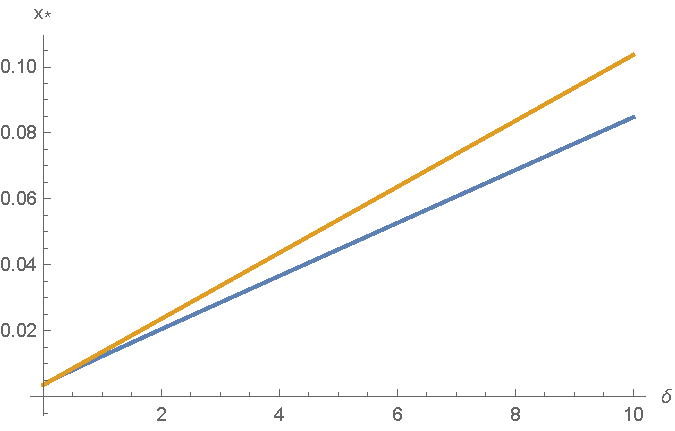
\includegraphics[width=0.45\textwidth]{Prob2_CapOpt/xopt_delta.pdf}}
		\subfigure[$\sigma \in (0,1)$]{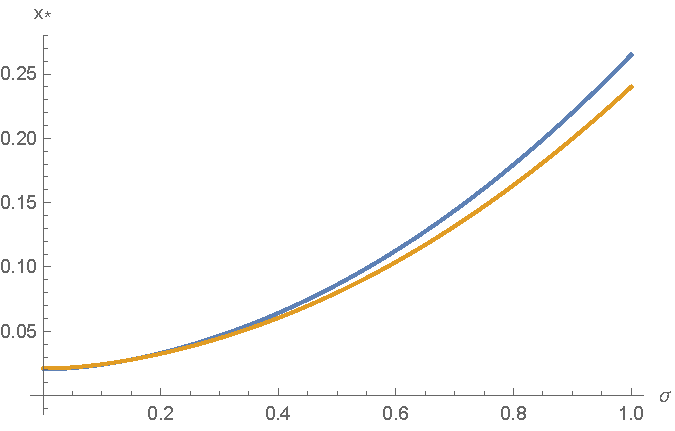
\includegraphics[width=0.45\textwidth]{Prob2_CapOpt/xopt_sigma.pdf}}
	\end{subfigmatrix}
	\caption{Threshold value with respect to the benchmark model (orange) and the capacity optimized model (blue) and parameters with which $x^*_B$ increases.}
	\label{fig:2_x2}
\end{figure}

On Figure \ref{fig:2_x2}, we obtained similar results to the ones on Section 2. Both threshold values increase with sensibility parameter $\delta$ and volatility $\sigma$. The first one is justified by the fact that a higher $\delta$ means a bigger investment, and thus it will only be made, if there's also a huge demand of the product. The second one is justified by the huge uncertainty of the demand. Since it has a high variance, the demand has a great amplitude of values, which delays the investment decision, only made when the demand reaches a high level. This is in accordance to what is described in \cite{dixit:book}.


\begin{figure}[!htb]
	\begin{subfigmatrix}{2}
		\subfigure[$\mu \in ( -r,r )$ ]{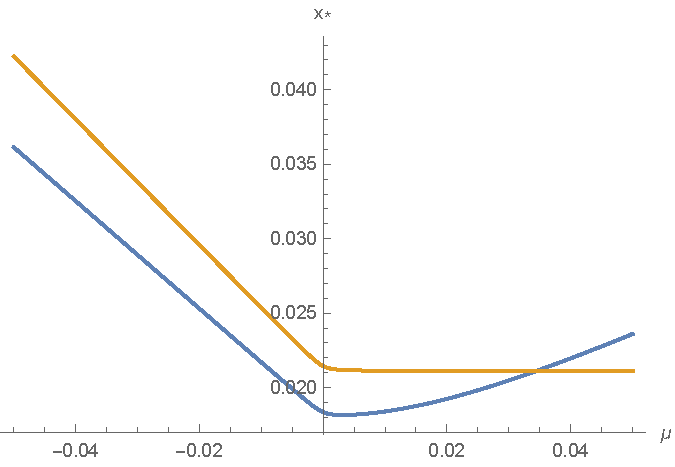
\includegraphics[width=0.45\textwidth]{Prob2_CapOpt/xopt_mu.pdf}}
		\subfigure[$\theta \in (1,10)$]{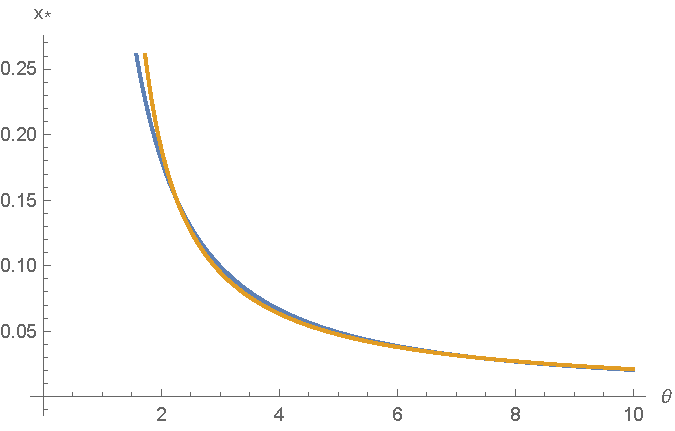
\includegraphics[width=0.45\textwidth]{Prob2_CapOpt/xopt_theta.pdf}}
	\end{subfigmatrix}
	\caption{Threshold value with respect to the benchmark model (orange) and the capacity optimized model (blue) and parameter with which  $x^*_B$ decreases.}
	\label{fig:2_x3}
\end{figure}

On Figure \ref{fig:2_x3} we see that similarly to what happened on Section 2, both threshold levels decrease with innovation level. Although the threshold level associated to the benchmark model decreases with $\mu$ in what seems to be a linear way for negative values of $\mu$ and almost negligible for positive values of $\mu$, the same doesn't happen to the threshold level associated to the capacity optimization model. This last one, seems to increase for positive values of $\mu$. The same happened considering other values for parameters $K_0, \ \alpha, \ \delta, \ \theta$. Regarding $\sigma$, we obtained that when increasing the volatility, the value of $\mu$ associated wityh the stationary point happens for values of $\mu$ greater than 0.

\begin{figure}[!htb]
	\begin{subfigmatrix}{2}
		\subfigure[$r \in (\mu,1)$, $\mu=0.01$ and $\sigma=0.9$]{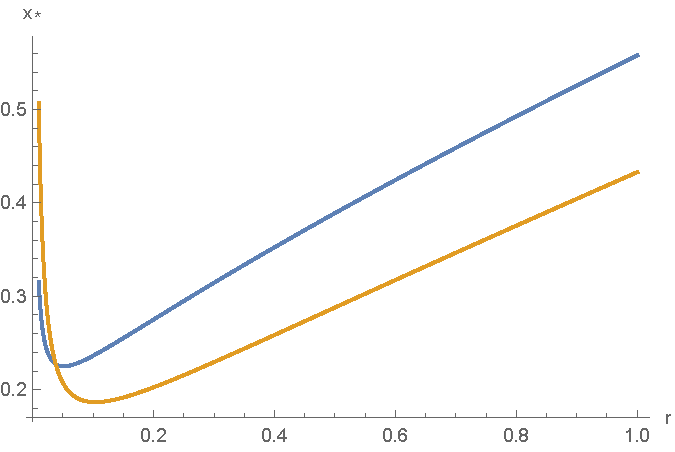
\includegraphics[width=0.45\textwidth]{Prob2_CapOpt/xopt_r.pdf}}
		\subfigure[$K_0 \in ( 0, \frac{1}{\alpha}=100 )$ ]{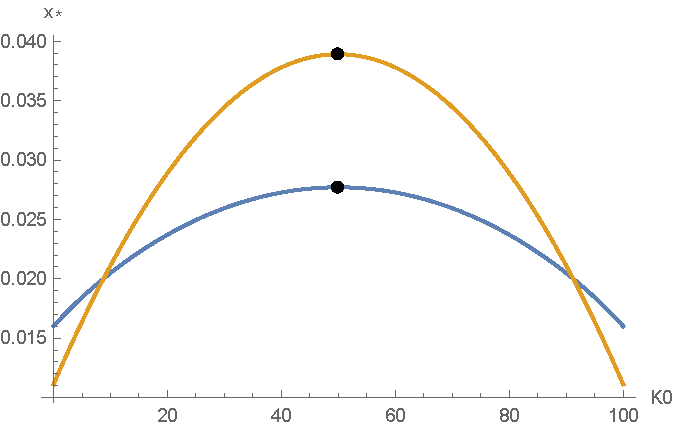
\includegraphics[width=0.45\textwidth]{Prob2_CapOpt/xopt_k0.pdf}}
		\subfigure[$K_1 \in (0, \frac{\theta}{\alpha}=1000 )$]{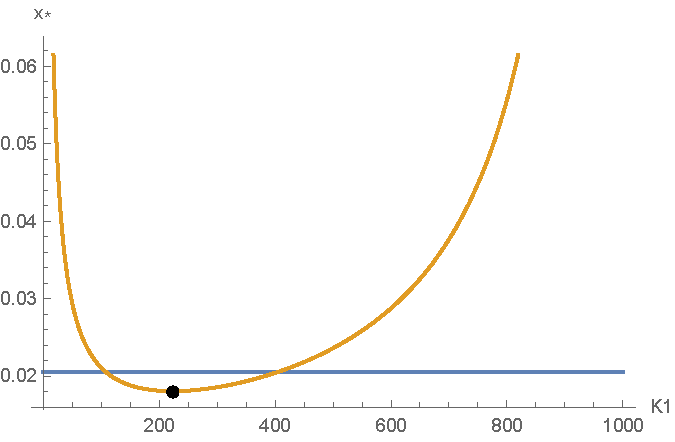
\includegraphics[width=0.45\textwidth]{Prob2_CapOpt/xopt_k1.pdf}}
	\end{subfigmatrix}
	\caption{Threshold value with respect to the benchmark model (orange) and the capacity optimized model (blue) and parameters with which  $x^*_B$ has a non-monotonic behaviour.}
	\label{fig:2_x1}
\end{figure}

On Figure \ref{fig:2_x1}, we observe that both threshold level behave in a non-monotonic way with $r$ and $K_0$.

Interestingly, a maximum value is observed when the capacity level of the \textit{older} product is exactly equal to $\frac{1}{2 \alpha}$, whose value comes from the expression $\alpha K_0 \pi_0=\alpha K_0 (1-\alpha K_0)$ included on both expressions of $x_B^*$ \eqref{} and $x^*_C$ \eqref{}.

Regarding parameter $K_1$, its value doesn't affect threshold $x^*_C$, since it takes into account the optimal capacity $K^*_C$. However, when it comes to the threshold $x^*_B$ we have that it achieves a minimum value at $K_1=\frac{\pi_0+\sqrt{\alpha \pi_0(\pi_0+\delta \theta r)}}{r\alpha \delta}$, as it's represented on the bottom plot.
	
	\begin{figure}[!htb]
		\begin{subfigmatrix}{2}
			\subfigure[$\alpha \in (0,1)$$\theta=10>\frac{K_1}{ K_0^2} (K_0+K_1 r \delta)$]{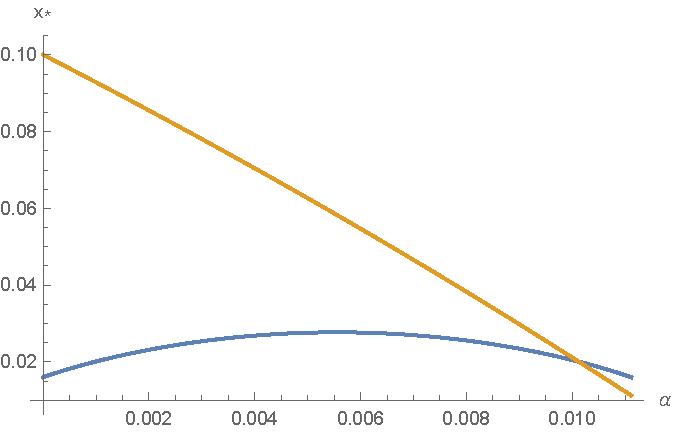
\includegraphics[width=0.45\textwidth]{Prob2_CapOpt/xopt_alpha.pdf}}
			\subfigure[$\alpha \in (0,1) $ and $\theta=1<\frac{K_1}{ K_0^2} (K_0+K_1 r \delta)$]{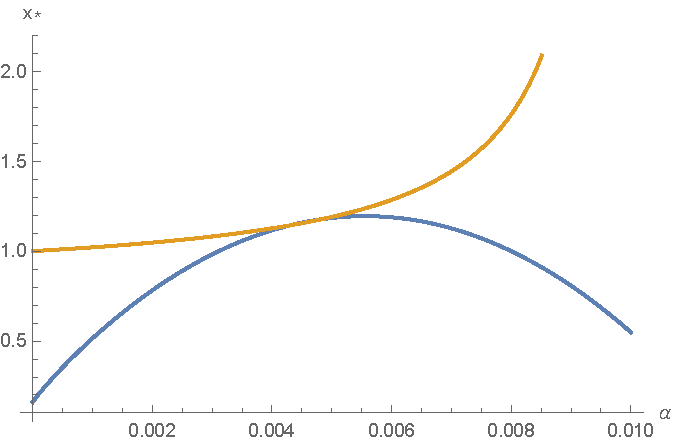
\includegraphics[width=0.45\textwidth]{Prob2_CapOpt/xopt_alpha_o1.pdf}}
		\end{subfigmatrix}
		\caption{Threshold value with respect to the benchmark model (orange) and the capacity optimized model (blue) and sensibility parameter $\alpha$.}
		\label{fig:2_x4}
	\end{figure}
	
	On Figure \ref{fig:2_x4} it's represented the behaviour of $x^*_B$ with $\alpha$, as written on Proposition (???). Considering fixed values mentioned in REFERIRRRR, we obtain a $\theta$-threshold equal to $\frac{K_1}{ K_0^2} (K_0+K_1 r \delta)=1.23457$. Testing for innovation levels smaller and greater than the mentioned threshold, we verify what was deduced: that $x^*_C$ behaves differently with $\alpha$ for certain levels of innovation.
	
	Note that on most of the plots you have that the threshold $x_C^*$ has an associated capacity level ($K^*(x_C^*)$) greater than the one considered ($K_1=100$), resulting in values $x^*_B$ smaller than $x_C^*$, contrarily to what happened on the previous section.
	\vspace{2cm}
	
	Now we analyse optimal capacity level $K^*_C$, that is given by evaluating $K^*$ as defined in \eqref{ass3} on demand level $x^*_C$, as done in \cite{huis:cap} and in the previous section. Its expression is given by
$$K^*_C=\frac{\theta }{2 \alpha }-\frac{\delta  (d_1-1) \theta ^2 r}{2 \alpha  \left(\sqrt{4 \alpha  d_1^2 \pi_0 (\alpha  \pi_0+\delta  \theta  r)+\delta ^2 \theta ^2 r^2}+d_1 (2 \alpha  \pi_0+\delta  \theta  r)\right)}.$$\\

\textbf{Proposition:}
Optimal capacity level $K^*_C$ increases asymptotically with $\theta$ and does not have a monotonic behaviour with $K_0$. Also, 

\textbf{Proof:}

Regarding innovation level $\theta$, assuming that it has no upper limit, it's possible to evaluate its behaviour asymptotically. Denoting $\theta_K:=\frac{\sigma ^2 \left(\sqrt{\delta ^2 r^2}+\delta  r\right)}{\alpha  \left(2 \sigma ^2 \sqrt{\delta ^2 r^2}+\delta  r \left(\sigma ^2 (\phi +1)-2 \mu \right)\right)}>0$, we obtain that $K^*_C$ increases on order of $\theta_K \theta$, that is,
$$K^*_C(\theta) \sim \theta_K \theta \ \Leftrightarrow \ \lim_{\theta \to \infty}  \frac{K^*_C}{\theta_K \theta}=1 $$


The non monotonic behaviour of $K^*_C$ with $K_0$ will be showed hereunder in the obtained plots.
\begin{flushright}
	$\square$
\end{flushright}

Although it wasn't possible to derive any (strong) analytical solution about te behaviour of the other parameters, numerically we obtain robust results. By manipulating each parameter, using command \texttt{Manipulate}, we obtained no different behaviours from the ones showed hereunder.

The results obtained regarding parameters $\mu, \ \sigma,\ r, \ \alpha$ and $\theta$  were similar to the ones obtain for the optimal capacity level on the previous section.  Since $K^*_C$ depends on value $x_C^*$, it is expected to observe similiar behaviours regarding the studied parameters. 

Starting with the capacity level of the \textit{old} product $K_0$ and respective considered parameters, on Figure \ref{fig:2_k0}, we obtained that the highest optimal capacity level $K^*_C$ happens for $K_0=\frac{1}{2 \alpha}$. This is motivated by the results obtained for $x^*_C$, as seen on Figure \ref{fig:},which also reaches its highest value at $\frac{1}{2 \alpha}$.

\begin{figure}[!htb]
	\centering
	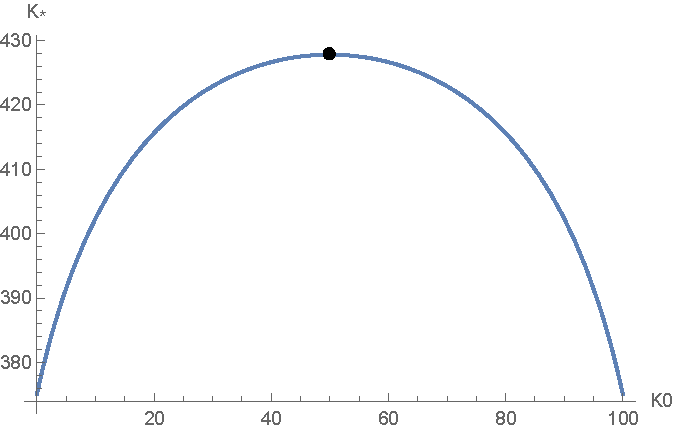
\includegraphics[width=0.45\textwidth]{Prob2_CapOpt/koptx_k0.pdf}
	\caption{Optimal capacity regarding the threshold value $x^*_C$ considering capacity levels $K_0 \in [0, 100)$ and its highest values at $\frac{1}{2 \alpha}=50$.}
	\label{fig:2_k0}
\end{figure}

On Figure \ref{fig:2_k1}, we obtain that $K^*_C$ increases with both drift and volatility, as it happened in the previous section. Note that again that, contrary to what happens for positive drift values, the growth of $K^*_C$ with $\mu$ is barely noticeable for negative values of $\mu$.
%Recall that the demand process evolves accordingly to a GBM and its expected value at time $t$ is given by $\textbf{E}^{X_0=x_0} [X_t]=x_0 e^{\mu t}$.

\begin{figure}[!htb]
	\begin{subfigmatrix}{2}
		\subfigure[$\mu \in ( -r,r )$ ]{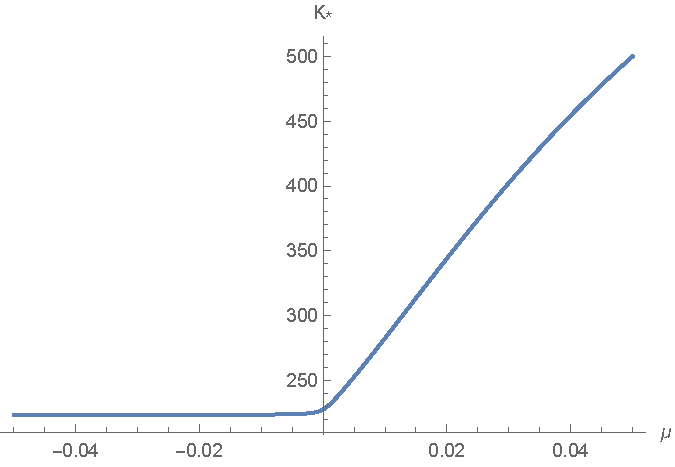
\includegraphics[width=0.45\textwidth]{Prob2_CapOpt/koptx_mu.pdf}}
		\subfigure[$\sigma \in (0,1)$]{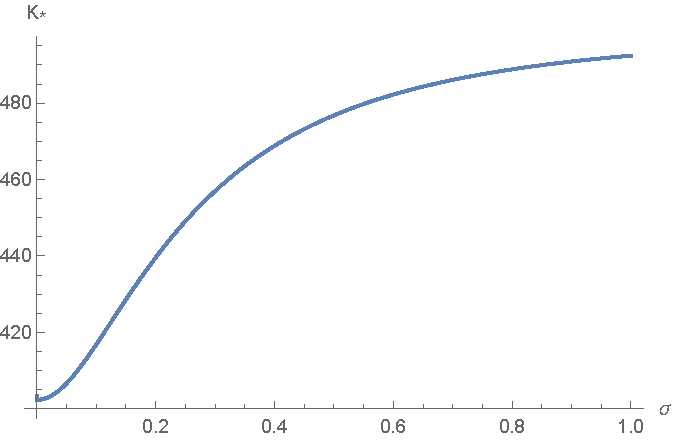
\includegraphics[width=0.45\textwidth]{Prob2_CapOpt/koptx_sigma.pdf}}
	\end{subfigmatrix}
	\caption{Optimal capacity regarding the threshold value $x^*_C$.}
	\label{fig:2_k1}
\end{figure}

Regarding innovation level $\theta$ and sensibility parameter $\delta$, we have on Figure \ref{fig:2_k3} that $K^*_C$ increases with them as well. Note that asymptotically, $K^*_C$ seems to increase linearly with $\theta$, as previously deduced.

\begin{figure}[!htb]
	\begin{subfigmatrix}{2}
		\subfigure[$ \theta \in ( 1, 10 )$]{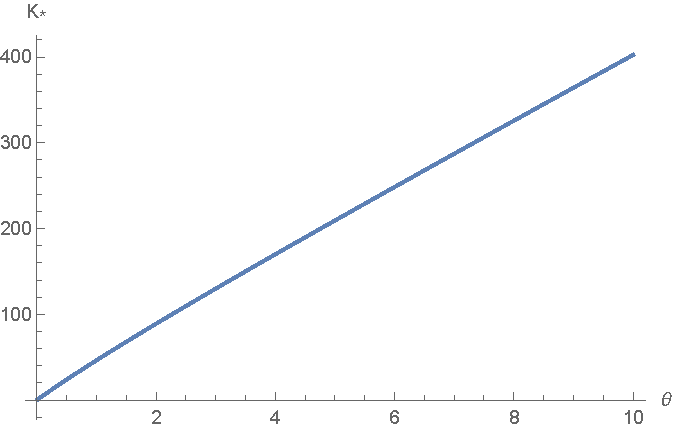
\includegraphics[width=0.45\textwidth]{Prob2_CapOpt/koptx_theta.pdf}}
		\subfigure[$ \delta \in (0,10)$]{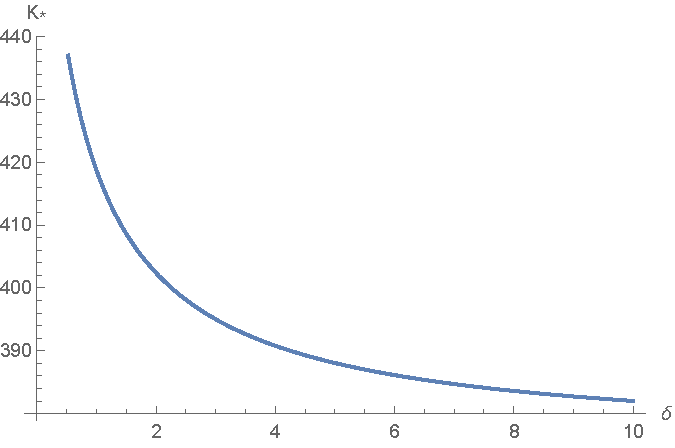
\includegraphics[width=0.45\textwidth]{Prob2_CapOpt/koptx_delta.pdf}}
	\end{subfigmatrix}
	\caption{Optimal capacity regarding the threshold value $x^*_C$.}
	\label{fig:2_k3}
\end{figure}

Regarding discount rate $r$ and sensibility parameter $\alpha$, we have on Figure \ref{fig:2_k2} that $K^*_C$ decreases with them, as happened in the previous section.

\begin{figure}[!htb]
	\begin{subfigmatrix}{2}
		\subfigure[$ r \in ( \mu, 1 )$]{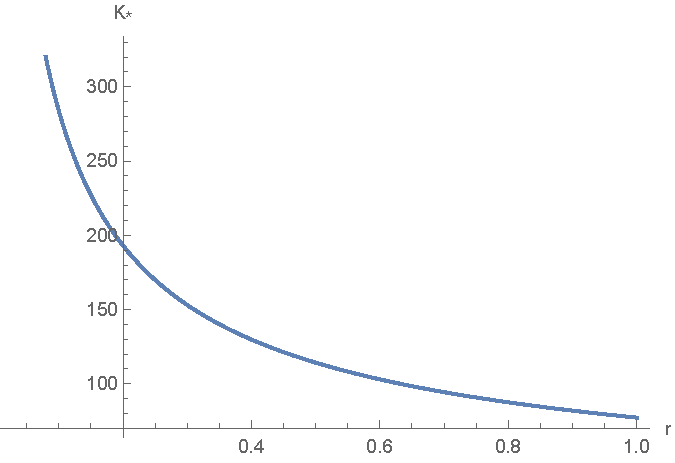
\includegraphics[width=0.45\textwidth]{Prob2_CapOpt/koptx_r.pdf}}
		\subfigure[$ \alpha \in (0,1)$]{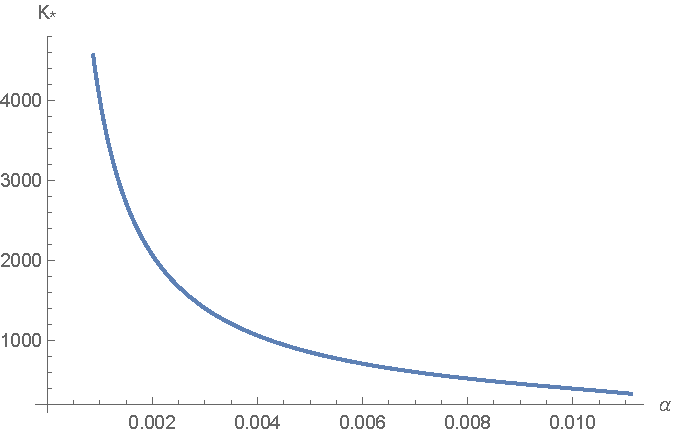
\includegraphics[width=0.45\textwidth]{Prob2_CapOpt/koptx_alpha.pdf}}
	\end{subfigmatrix}
	\caption{Optimal capacity regarding the threshold value $x^*_C$.}
	\label{fig:2_k2}
\end{figure}